\section{Introduction}
The success of any complex software-intensive system is dependent on how effectively it addresses the stakeholder's quality attribute concerns such as security, usability, availability, and interoperability. Designing a system to satisfy these concerns involves devising and comparing alternate solutions, understanding their trade-offs, and ultimately making a series of design choices. These architectural decisions typically begin with design primitives such as architectural tactics and patterns.

Tactics are the building blocks of architectural design~\cite{bass:arch12}, reflecting the fundamental choices that an architect makes to address a quality attribute concern. Architectural tactics come in many different shapes and sizes and describe solutions for a wide range of quality concerns. They are particularly prevalent across high-performance and fault tolerant software systems. Reliability tactics such as Redundancy with Voting, Heartbeat, and Check-Pointing provide solutions for fault mitigation, detection, and recovery; while performance tactics such as Resource Pooling and Scheduling help optimize response time and latency.


%% When the paper gets accepted, change the wording to no long refer to ourselves in the 3rd person

%%% Build up the previous study and show how important/profound it was. This will make our work seem more important

The importance of rigorously and robustly implementing architectural tactics was highlighted by a small study that was conducted in a previous work that investigated tactic implementations in Hadoop and OFBiz and evaluated their degree of stability during the maintenance process~\cite{MSRBuble}. For each of these projects we retrieved a list of bug fixes from the change logs (Nov. 2008 - Nov. 2011 for Hadoop, and Jan. 2009 - Nov. 2011 for OFBiz). Our analysis showed that tactics-related classes incurred 2.8 times as many bugs in Hadoop, and 2.0 times as many bugs in OFBiz as non-tactics related classes. These observations suggest that tactic implementations, if not developed correctly, are likely to contribute towards the well-documented problem of architectural degradation~\cite{Erosion}. Less experienced developers sometimes find this challenging, primarily because of the variability points that exist in a tactic, and the numerous design decisions that need to be made in order to implement a tactic in a robust and effective way. We found many examples of such questions on coding forums.

%\begin{figure}[tbph]
%\centering
%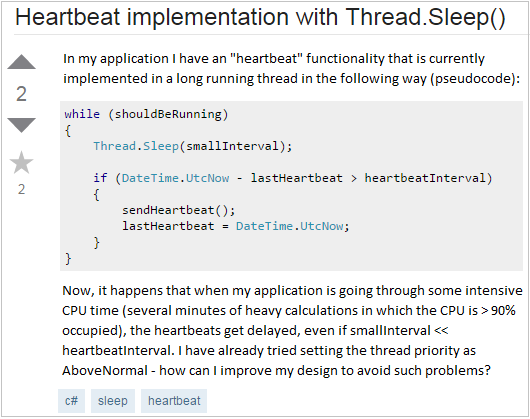
\includegraphics[width=0.99\linewidth]{./img/Question}
%\caption{}
%\label{fig:Question}
%\end{figure}


A robust tactic  search engine that shares sample code snippets from successful implementation of tactics in open source community can provide valuable support for the developers.


%%%% DK: I removed this to protect blind review 9/19/15
% In a previous paper we presented the overall architecture of such search engine~\cite{BIGSE}. 

The primary contributions of this paper are: 
%% DK: I put these into a list since I thought it would make it really clear what our contributions were and make them easy to read

\begin{enumerate}
   \setlength{\itemsep}{0pt} %Cut down on spacing for the different items in the list
   \setlength{\parskip}{0pt} %Cut down on spacing for the different items in the list
   \setlength{\parsep}{0pt}  %Cut down on spacing for the different items in the list

  \item Reporting the \textit{results of a qualitative code review study} conducted to identify challenges in implementing architectural tactics and \textit{reusing tactical code}.
  \item Identifying the foundations of a practical tactic search engine.
  \item Introducing the notion of \textit{tactical clones} and formulating the next steps in realizing tactic search engine.
\end{enumerate}


%A) Reporting the \textit{results of a qualitative code review study} conducted to identify challenges in implementing architectural tactics and \textit{reusing tactical code}. B) Identifying the foundations of a practical tactic search engine. C) Introducing the notion of \textit{tactical clones} and formulating the next steps in realizing tactic search engine.

Although there have been some initial development of source code recommender systems~\cite{DBLP:conf/icse/McMillanHPCM12,6340250}, the primary focus of these works are on generic code, and not tactical codes. Therefore the challenges of obtaining and recommending architecturally significant code is still unexplored. This paper focuses on identifying these challenges.

The structure of this paper is as the following.
Section~\ref{sec:Method} present the underlying methodology used to conduct the qualitative study of tactic implementation.  Section \ref{sec:SeenUnSeen} discusses the results of our qualitative study, tactic implementation issues, reusability concerns and other  observations across several implementation of architectural tactics. Furthermore this section summarizes the foundations for developing a practical tactic search engine. Section \ref{sec:Clones} presents the definitions of tactical clones and the process of extracting sample architectural clones from source code of several open source systems. Finally section \ref{sec:Future} presents the future work and section \ref{sec:Conclusion} is the conclusion.